\documentclass[11pt]{article}
\usepackage[margin=1in]{geometry}
\usepackage{setspace}
\usepackage{booktabs}
\usepackage{amsmath}
\usepackage{caption}
\usepackage[authoryear,round]{natbib}
\usepackage{threeparttable}
\usepackage{pgfplots}
\pgfplotsset{compat=1.17}
\usepackage[hidelinks]{hyperref}
\onehalfspacing
\captionsetup{font=small,labelfont=bf}

\title{Property Rights and the Research Workforce:\\ Examiner Assignment, Patent Grants, and Hiring in Velorian Firms\\[1em]
\normalsize\textbf{SYNTHETIC TEST PAPER, NOT REAL RESEARCH}}
\author{Author names withheld for review}
\date{}

\begin{document}
\maketitle

\begin{abstract}
\noindent Do patent grants change how firms build their research workforce? We study 12,480 patent applications filed at the Velorian Patent and Trademark Office between 2009 and 2015 and link applicant firms to the Velorian Employer-Employee Register. Because applications are assigned to examiners by docket rotation within art units, the leniency of the examiner an application draws shifts its chance of being granted for reasons unrelated to the firm. Using examiner leniency as an instrument for grant, we find that a patent grant raises the number of research and development (R\&D) employees the applicant hires over the following three years by about 23 percent. The effect is a local one for applications whose fate turns on the examiner, which come disproportionately from small and first-time applicants. A second analysis instruments firm R\&D spending with regional tax-credit changes and tariff cuts on laboratory equipment and finds that the hiring response to R\&D is stronger in venture-backed firms. Together the results suggest that secure property rights, and not only research budgets, shape the research labor market.
\end{abstract}

\section{Introduction}

Scholars of strategy and innovation have long argued that intellectual property rights let firms capture the returns to invention and so shape how much firms invest in knowledge work. A large body of work studies how patents affect financing, licensing, and firm growth. Much less is known about what patents do inside the firm, and in particular how a grant changes the firm's demand for the scientists and engineers who produce the next round of inventions. This question matters for the organization of innovative firms. If property rights raise the expected return to the firm's knowledge stock, a grant should lead firms to expand the research workforce that builds on it. If instead patents mainly serve as signals to outside investors, hiring may respond little, or only in firms that face tight financing constraints.

Estimating the effect of a patent grant on hiring is difficult because grants are not assigned at random. Firms that receive patents file better applications, employ better attorneys, and are often already growing. A simple comparison of granted and rejected applicants therefore mixes the effect of the grant with the qualities that produced it. We address this problem by exploiting the assignment of applications to examiners at the Velorian Patent and Trademark Office (VPTO). Within an art unit and filing year, applications are routed to examiners by docket rotation, and examiners differ in how readily they grant. The leniency of the examiner an application draws therefore changes its probability of grant for reasons outside the applicant's control.

Our data link 12,480 applications from 3,016 firms, examined by 214 examiners in 24 art units, to administrative employment records that identify each new hire's occupation. We measure the outcome as the number of R\&D employees the applicant firm hires in the three years after the examiner's final decision. Two-stage least squares (2SLS) estimates show that a grant raises three-year R\&D hiring by about 23 percent, an effect that is statistically significant at the 5 percent level and five times larger than the ordinary least squares (OLS) estimate. We show who the compliers are: applications from small firms and first-time applicants are over-represented among them, which frames the estimate as an effect for applicants whose grant turns on the examiner.

A second analysis moves from property rights to research inputs. Using regional changes in R\&D tax-credit rates and industry-level tariff cuts on laboratory equipment as instruments for firm R\&D spending, we estimate the hiring response to R\&D investment and find that it is stronger in venture-backed firms, where complementary financing is easier to obtain.

The paper makes two contributions. First, it provides quasi-experimental evidence that the grant decision itself, and not only the invention behind it, shapes the research workforce of the applicant. Second, it separates the hiring effect of property rights from the hiring effect of R\&D budgets and shows how financing conditions moderate the latter.

\section{Theory and Hypotheses}

\subsection{Patents and the demand for research labor}

A patent gives its holder the right to exclude others from practicing an invention for a fixed term. Strategy research treats this right as a mechanism of appropriability: it raises the share of an invention's value that the inventing firm can capture. When appropriability rises, the marginal value of complementary investments in the protected technology rises as well. Follow-on inventions, product development, and process improvements all build on the protected knowledge, and each requires scientists and engineers.

A grant can also change the firm's planning horizon. An application under examination leaves the firm uncertain about whether its core technology will be protected. Managers facing this uncertainty may delay hiring decisions that commit the firm to a technological trajectory. A grant resolves the uncertainty and allows the firm to commit resources, including long-term hiring, to the protected area. Both arguments predict that a grant raises the firm's hiring of R\&D personnel.

\begin{quote}
\textit{Hypothesis 1.} Receiving a patent grant increases the applicant firm's subsequent hiring of R\&D employees.
\end{quote}

\subsection{R\&D investment, financing, and hiring}

Research budgets and research personnel are complements, but the strength of the link depends on whether the firm can finance the fixed costs of expanding a team. Hiring scientists involves search costs, onboarding, and wage commitments that outlast any single project. Firms with access to outside equity can treat a rise in R\&D spending as a signal to scale the team. Firms without such access may instead spend additional R\&D funds on equipment, contracts, or existing staff. Venture-backed firms have both committed capital and investors who expect rapid scaling of technical teams, so their hiring should respond more strongly to R\&D investment.

\begin{quote}
\textit{Hypothesis 2.} The hiring response to R\&D investment is stronger in venture-backed firms than in other firms.
\end{quote}

\section{Setting: The Velorian Patent and Trademark Office}

The Republic of Veloria is a mid-sized industrial economy whose patent office, the VPTO, receives about 22,000 applications a year. Applications are classified by technology into art units. Within an art unit, a supervisory examiner routes incoming applications to examiners by docket rotation: each new application goes to the next examiner on the list, subject to workload caps. Applicants cannot choose their examiner and learn the examiner's identity only after assignment. An examiner who issues a final rejection can be appealed to the Velorian Patent Appeals Board, but appeals are costly and uncommon among the firms in our sample.

Every VPTO decision is reviewed by a second examiner before it becomes final. This quality-assurance step narrows the differences in grant rates across examiners relative to what is reported for larger offices. Nonetheless, examiners within the same art unit and year still differ in how often they grant, and these differences persist over time.

Granted patents can be challenged in opposition proceedings before the Appeals Board within five years of grant. Opposition outcomes are public, which lets us observe whether a granted patent is later invalidated.

\section{Data and Measures}

\subsection{Sample}

We start from the universe of VPTO applications filed between 2009 and 2015 by firms with a Velorian tax identifier. We link applicants to the Velorian Employer-Employee Register (VEER), which records every employment spell in the country together with an occupation code. We keep applications whose final decision was issued by 2017 so that three full years of post-decision hiring are observed through 2020. The resulting sample contains 12,480 applications from 3,016 firms, examined by 214 examiners in 24 art units.

\subsection{Measures}

\textit{R\&D hiring.} Our outcome is the number of new R\&D employees (occupation codes for scientists, engineers, and research technicians) that the applicant firm hires in the three years after the examiner's final decision. Because the count is skewed, we use $\log(1 + \text{hires})$.

\textit{Patent granted.} An indicator equal to one if the application was granted, taken from the VPTO decision record.

\textit{Examiner leniency.} We measure each examiner's leniency as the examiner's grant rate over all applications the examiner decided between 2009 and 2017, including the focal application. We residualize this grant rate on art unit by filing year indicators and standardize it to have mean zero and standard deviation one in the estimation sample. In raw terms, the residualized grant rate has a standard deviation of 1.6 percentage points.

\textit{Controls.} All models control for characteristics fixed at filing: the number of claims, the log of the firm's employment in the year of filing, firm age, the log of one plus the firm's prior VPTO applications, and indicators for small firms (fewer than 50 employees), first-time applicants, and venture capital backing.

\textit{R\&D panel.} For the second analysis we build a firm-year panel of 41,870 observations for 5,904 firms from 2009 to 2017, using R\&D spending reported to the Velorian statistical agency. The outcome is the same three-year R\&D hiring measure, computed from each firm-year forward. The instruments are the change in the R\&D tax-credit rate in the firm's district (Veloria has 48 districts, which set their own credit rates) and the cut in import tariffs on laboratory equipment used in the firm's industry (52 industries).

Table~\ref{tab:desc} reports descriptive statistics.

\begin{table}[htbp]
\centering
\begin{threeparttable}
\caption{Descriptive statistics, application sample}
\label{tab:desc}
\small
\begin{tabular}{lrrrr}
\toprule
Variable & Mean & SD & Min & Max \\
\midrule
R\&D hires, three years after decision & 6.8 & 14.2 & 0 & 412 \\
$\log(1 + \text{R\&D hires})$ & 1.21 & 1.05 & 0 & 6.02 \\
Patent granted & 0.582 & 0.493 & 0 & 1 \\
Examiner grant rate, residualized & 0.000 & 0.016 & $-0.058$ & 0.061 \\
Number of claims & 16.4 & 9.7 & 1 & 118 \\
$\log$ employment at filing & 3.94 & 1.61 & 0 & 10.21 \\
Firm age (years) & 14.2 & 11.8 & 0 & 96 \\
$\log(1 + \text{prior applications})$ & 1.37 & 1.12 & 0 & 6.84 \\
Small firm ($<$ 50 employees) & 0.385 & 0.487 & 0 & 1 \\
First-time applicant & 0.290 & 0.454 & 0 & 1 \\
Venture-backed & 0.170 & 0.376 & 0 & 1 \\
\bottomrule
\end{tabular}
\begin{tablenotes}\footnotesize
\item \textit{Notes:} $N = 12{,}480$ applications from 3,016 firms, 214 examiners, and 24 art units, filed 2009 to 2015. The examiner grant rate is residualized on art unit by filing year indicators; regressions use its standardized version.
\end{tablenotes}
\end{threeparttable}
\end{table}

\subsection{Examiner leniency and patent quality}

Table~\ref{tab:quart} and Figure~\ref{fig:inval} describe how outcomes vary across examiner leniency quartiles. Grant rates rise from 56.4 percent for the least lenient quartile to 60.1 percent for the most lenient. Patents granted by lenient examiners are also invalidated more often in later opposition proceedings: 9.6 percent of patents granted by examiners in the top leniency quartile are invalidated, compared with 4.3 percent in the bottom quartile. We read this pattern as further evidence that lenient examiners apply a lower bar for grant, which is the variation our instrument exploits.

\begin{table}[htbp]
\centering
\begin{threeparttable}
\caption{Grant and invalidation rates by examiner leniency quartile}
\label{tab:quart}
\small
\begin{tabular}{lcccc}
\toprule
 & Q1 (least lenient) & Q2 & Q3 & Q4 (most lenient) \\
\midrule
Applications & 3,121 & 3,118 & 3,122 & 3,119 \\
Grant rate & 0.564 & 0.577 & 0.586 & 0.601 \\
Share of granted patents later invalidated & 0.043 & 0.056 & 0.074 & 0.096 \\
\bottomrule
\end{tabular}
\begin{tablenotes}\footnotesize
\item \textit{Notes:} Quartiles of the residualized examiner grant rate within the estimation sample. Invalidation is measured by opposition proceedings at the Velorian Patent Appeals Board within five years of grant.
\end{tablenotes}
\end{threeparttable}
\end{table}

\begin{figure}[htbp]
\centering
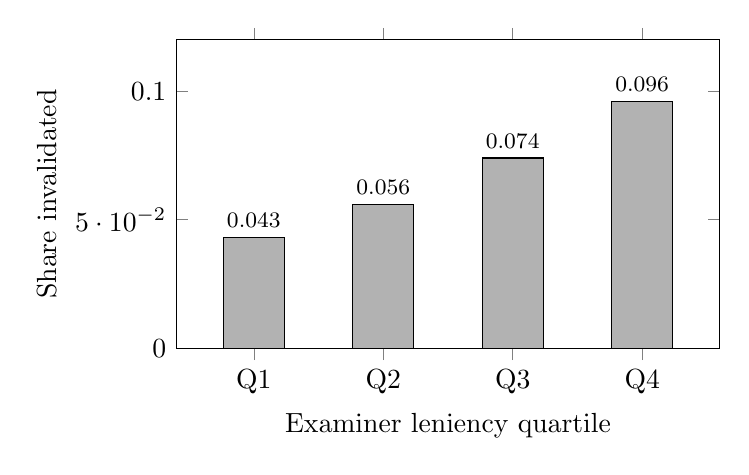
\begin{tikzpicture}
\begin{axis}[
  ybar, width=0.7\textwidth, height=5.5cm,
  symbolic x coords={Q1,Q2,Q3,Q4},
  xtick=data, ymin=0, ymax=0.12,
  ylabel={Share invalidated},
  xlabel={Examiner leniency quartile},
  nodes near coords, nodes near coords style={font=\footnotesize, /pgf/number format/fixed, /pgf/number format/precision=3},
  bar width=22pt, enlarge x limits=0.2]
\addplot[fill=gray!60] coordinates {(Q1,0.043) (Q2,0.056) (Q3,0.074) (Q4,0.096)};
\end{axis}
\end{tikzpicture}
\caption{Share of granted patents later invalidated in opposition proceedings, by examiner leniency quartile. Source: Table~\ref{tab:quart}.}
\label{fig:inval}
\end{figure}

\section{Empirical Strategy}

We estimate the effect of a grant on hiring with the model
\begin{equation}
\log(1 + \text{Hires}_{i}) = \beta\,\text{Granted}_{i} + X_{i}'\gamma + \alpha_{u(i)t(i)} + \varepsilon_{i},
\end{equation}
where $i$ indexes applications, $X_i$ contains the controls listed above, and $\alpha_{ut}$ are art unit by filing year fixed effects, which define the stratum within which docket rotation assigns examiners. Grant is instrumented with the standardized leniency of the application's examiner, $Z_i$, in the first stage
\begin{equation}
\text{Granted}_{i} = \pi Z_{i} + X_{i}'\delta + \mu_{u(i)t(i)} + \nu_{i}.
\end{equation}
Standard errors are two-way clustered by examiner (214 clusters), the level at which the instrument is assigned, and by applicant firm (3,016 clusters).

Three assumptions give $\beta$ a causal reading \citep{imbens1994}. The first is relevance: examiner leniency must shift grant. The second is exclusion: the examiner an application draws must affect hiring only through the grant decision. We consider the channels through which an examiner could affect the applicant other than through grant. Examiners differ in how long they take, but the decision date anchors our outcome window, so slower examination shifts the window rather than shortening it. Examiners can also narrow claims before grant; we return to claim scope below. Finally, examiner identity is not disclosed to investors or recruits in any systematic way before the decision. As a falsification test, we estimate the model with hiring in the three years \textit{before} filing as the outcome; a grant decided years later should not predict it. The third assumption is monotonicity: an application granted by a strict examiner would also be granted by a more lenient one. We probe this assumption by estimating the first stage separately for subgroups of applicants and checking that it is positive in each (Section~\ref{sec:compliers}).

\section{Results}

\subsection{Main estimates}

Table~\ref{tab:main} reports the main results. Column (1) shows the OLS estimate. Granted applicants hire more R\&D workers than rejected applicants in the same art unit and year, by about 4 percent (coefficient 0.041, standard error 0.008).

Column (2) reports the 2SLS estimate. The first stage is positive: a one standard deviation increase in examiner leniency raises the probability of grant by 1.41 percentage points (Appendix Table~\ref{tab:fs}). The Cragg-Donald F = 11.3, above the Stock-Yogo 15 percent maximal size critical value of 8.96 \citep{cragg1993,stock2005}, so weak instruments are not a concern in our setting. The 2SLS coefficient is 0.205 with a standard error of 0.089 ($p = 0.021$). A grant thus raises three-year R\&D hiring by about 23 percent ($e^{0.205} - 1 = 0.23$), and the effect is significant at the 5 percent level. This result supports Hypothesis 1.

The 2SLS estimate is five times the OLS estimate. We attribute this gap to the instrument correcting measurement error in the grant indicator, which attenuates the OLS coefficient toward zero. Once this error is purged, the effect of property rights on hiring is considerably larger than naive comparisons suggest.

\begin{table}[htbp]
\centering
\begin{threeparttable}
\caption{Patent grant and subsequent R\&D hiring: OLS and 2SLS estimates}
\label{tab:main}
\small
\begin{tabular}{lcc}
\toprule
 & (1) & (2) \\
 & OLS & 2SLS \\
\midrule
Patent granted & 0.041*** & 0.205** \\
 & (0.008) & (0.089) \\[0.5em]
Controls at filing & Yes & Yes \\
Art unit $\times$ filing year FE & Yes & Yes \\
Instrument & & Examiner leniency \\
Cragg-Donald F & & 11.3 \\
Mean of dependent variable & 1.21 & 1.21 \\
Observations & 12,480 & 12,480 \\
Examiner clusters & 214 & 214 \\
Firm clusters & 3,016 & 3,016 \\
\bottomrule
\end{tabular}
\begin{tablenotes}\footnotesize
\item \textit{Notes:} The dependent variable is $\log(1 + \text{R\&D hires})$ in the three years after the final decision. Standard errors in parentheses are two-way clustered by examiner and applicant firm. *** $p<0.01$, ** $p<0.05$, * $p<0.10$.
\end{tablenotes}
\end{threeparttable}
\end{table}

\subsection{Who are the compliers?}
\label{sec:compliers}

The 2SLS estimate is a local average treatment effect: it measures the effect of a grant for compliers, the applications that would be granted by a lenient examiner but not by a strict one \citep{imbens1994}. Compliers cannot be identified individually, but their observable traits can be described. For a binary characteristic, the ratio of the first-stage coefficient in the subgroup with the characteristic to the first-stage coefficient in the full sample gives the relative likelihood that a complier has that characteristic, and multiplying this ratio by the subgroup's sample share gives the share of compliers in the subgroup.

Table~\ref{tab:compliers} reports these calculations. Small firms make up 38.5 percent of the sample but 60.8 percent of compliers; the first stage for small firms is 0.0223, or 1.58 times the full-sample first stage of 0.0141. First-time applicants make up 29.0 percent of the sample and 40.9 percent of compliers. Venture-backed firms are slightly under-represented among compliers (12.9 percent against 17.0 percent of the sample). The first stage is positive in every subgroup, which is consistent with monotonicity.

These patterns fit the institutional setting. Small and first-time applicants rarely appeal and often lack in-house patent counsel, so for them the examiner's decision is more often the last word. Our estimate should therefore be read as the effect of a grant for applicants of this kind, whose grant turns on the examiner they draw. We do not claim that it is the average effect of a grant for all applicants, and in particular it says little about large, experienced applicants whose applications would be granted or rejected whichever examiner they drew.

\begin{table}[htbp]
\centering
\begin{threeparttable}
\caption{Characteristics of compliers}
\label{tab:compliers}
\small
\begin{tabular}{lcccc}
\toprule
 & Sample share & First stage & Relative likelihood & Complier share \\
 & (1) & (2) & (3) = (2)/0.0141 & (4) = (1) $\times$ (3) \\
\midrule
Full sample & 1.000 & 0.0141 & 1.00 & 1.000 \\[0.3em]
Small firm & 0.385 & 0.0223 & 1.58 & 0.608 \\
Not small & 0.615 & 0.0090 & 0.64 & 0.394 \\[0.3em]
First-time applicant & 0.290 & 0.0199 & 1.41 & 0.409 \\
Prior applicant & 0.710 & 0.0117 & 0.83 & 0.589 \\[0.3em]
Venture-backed & 0.170 & 0.0107 & 0.76 & 0.129 \\
Not venture-backed & 0.830 & 0.0148 & 1.05 & 0.872 \\
\bottomrule
\end{tabular}
\begin{tablenotes}\footnotesize
\item \textit{Notes:} Column (2) reports the first-stage coefficient on standardized examiner leniency estimated within each subgroup, with the controls and fixed effects of Table~\ref{tab:main}. Complier shares within each pair sum to one up to rounding.
\end{tablenotes}
\end{threeparttable}
\end{table}

\subsection{Falsification test and claim scope}

If lenient examiners were assigned to applicants that were already hiring more, the instrument would predict hiring before the application was filed. It does not. Estimating the 2SLS model with $\log(1 + \text{R\&D hires})$ in the three years before filing as the outcome gives a coefficient of 0.012 with a standard error of 0.084, far from the main estimate and not distinguishable from zero.

Examiners could also affect hiring by shaping claim scope, since a patent with broader claims may protect more of the firm's technology. Among granted applications, the number of claims at grant does not differ meaningfully across leniency quartiles (15.1 in the bottom quartile and 15.4 in the top quartile). We therefore treat grant as the main channel through which the examiner affects the applicant.

\subsection{R\&D investment and hiring}

Table~\ref{tab:rd} turns to the second analysis, in which firm R\&D spending is the endogenous variable. Column (1) reports OLS: a 10 percent increase in R\&D spending is associated with about 1 percent more R\&D hiring over three years (0.097, standard error 0.012). Standard errors in this table are two-way clustered by district (48 clusters) and industry (52 clusters), the levels at which the two instruments vary.

Columns (2) and (3) use one instrument at a time. With the tax-credit instrument alone in column (2), the Kleibergen-Paap rk Wald F = 21.4, above the Stock-Yogo 10 percent maximal size critical value of 16.38 \citep{kleibergen2006,stock2005}, and the 2SLS coefficient is 0.118 (standard error 0.041).

With the tariff instrument alone in column (3), the robust Kleibergen-Paap F is 38.0. With a single instrument this statistic equals the effective F of \citet{olea2013}, and it exceeds their critical value of 23.1 for a 5 percent test that the worst-case bias exceeds 10 percent of the benchmark. The 2SLS coefficient is 0.142 (standard error 0.033). Anderson-Rubin confidence intervals \citep{anderson1949}, reported at the bottom of the table, exclude zero in both columns.

Column (4) uses both instruments. The effective F is 26.4, again above the critical value of 23.1. The coefficient is 0.133 (standard error 0.026), between the two just-identified estimates. The Hansen J test (p = 0.42) confirms that our instruments are valid \citep{hansen1982}.

Column (5) tests Hypothesis 2 by adding the interaction of log R\&D spending with the venture-backed indicator, instrumented with the interaction of the tariff instrument with the same indicator. With two endogenous regressors, a single F for the system does not show whether each is separately identified, so we report the cluster-robust Sanderson-Windmeijer conditional F \citep{sanderson2016} for each endogenous term: 34.2 for log R\&D spending and 29.5 for its interaction with venture backing. Both exceed the Stock-Yogo value of 16.38 for one excluded instrument per endogenous term. The interaction coefficient is 0.068 (standard error 0.029, $p = 0.019$): the hiring response to R\&D spending is about 56 percent larger in venture-backed firms (0.068 relative to 0.121). This result supports Hypothesis 2.

\begin{table}[htbp]
\centering
\begin{threeparttable}
\caption{R\&D spending and subsequent R\&D hiring}
\label{tab:rd}
\footnotesize
\setlength{\tabcolsep}{4pt}
\begin{tabular}{lccccc}
\toprule
 & (1) & (2) & (3) & (4) & (5) \\
 & OLS & 2SLS & 2SLS & 2SLS & 2SLS \\
\midrule
\multicolumn{6}{l}{\textit{Panel A. Dependent variable: $\log(1 + \text{R\&D hires})$, next three years}} \\
$\log$ R\&D spending & 0.097*** & 0.118*** & 0.142*** & 0.133*** & 0.121*** \\
 & (0.012) & (0.041) & (0.033) & (0.026) & (0.036) \\
$\log$ R\&D spending $\times$ venture-backed & & & & & 0.068** \\
 & & & & & (0.029) \\[0.5em]
\multicolumn{6}{l}{\textit{Panel B. First stage. Dependent variable: $\log$ R\&D spending}} \\
Tax-credit rate change (pp) & & 0.046*** & & 0.043*** & \\
 & & (0.010) & & (0.010) & \\
Tariff cut on lab equipment (pp) & & & 0.031*** & 0.029*** & 0.030*** \\
 & & & (0.005) & (0.005) & (0.005) \\[0.5em]
\multicolumn{6}{l}{\textit{Diagnostics}} \\
Kleibergen-Paap rk Wald F & & 21.4 & 38.0 & & \\
Effective F (Montiel Olea-Pflueger) & & & 38.0 & 26.4 & \\
Cluster-robust conditional F, $\log$ R\&D & & & & & 34.2 \\
Cluster-robust conditional F, interaction & & & & & 29.5 \\
Hansen J p-value & & & & 0.42 & \\
Anderson-Rubin 95\% CI & & [0.029, 0.214] & [0.071, 0.216] & [0.077, 0.192] & \\[0.5em]
Firm and year FE & Yes & Yes & Yes & Yes & Yes \\
Observations & 41,870 & 41,870 & 41,870 & 41,870 & 41,870 \\
Firms & 5,904 & 5,904 & 5,904 & 5,904 & 5,904 \\
District / industry clusters & 48 / 52 & 48 / 52 & 48 / 52 & 48 / 52 & 48 / 52 \\
\bottomrule
\end{tabular}
\begin{tablenotes}\footnotesize
\item \textit{Notes:} Firm-year panel, 2009 to 2017. Column (5) instruments the interaction with the tariff instrument interacted with the venture-backed indicator; the venture-backed main effect is absorbed by the firm fixed effects because backing status is fixed within firm in our data. Standard errors in parentheses are two-way clustered by district and industry. *** $p<0.01$, ** $p<0.05$, * $p<0.10$.
\end{tablenotes}
\end{threeparttable}
\end{table}

\section{Discussion}

Our results suggest that the grant decision itself changes how applicant firms build their research workforce. Applicants that draw a lenient examiner, and are granted as a result, hire more R\&D staff over the following three years. The compliers are concentrated among small and first-time applicants, for whom a grant is often the first secure claim on their core technology. For the applicants whose grant turns on the examiner, property rights appear to relax the uncertainty that holds back long-term commitments to a technological trajectory.

The second analysis shows that research budgets also raise hiring, and more so in venture-backed firms. The contrast between the two analyses is informative. A grant raises hiring even holding the underlying invention fixed, which suggests that the value of the right to exclude, and not only the resources devoted to research, shapes the demand for research labor.

The results have implications for managers and for policy. For managers in small technology firms, the timing of hiring decisions may reasonably follow the resolution of patent examination. For patent offices, differences across examiners are not only a question of fairness among applicants: they shape the research employment of the firms whose applications are close calls.

Several limitations deserve mention. Our outcome covers hiring and not the productivity of the workers hired. The VPTO's second-examiner review compresses differences in grant rates across examiners, which limits the variation we can use. And the setting is a single office in a mid-sized economy; offices with different examination procedures may produce different compliers.

\section{Conclusion}

Using the assignment of patent applications to examiners at the Velorian Patent and Trademark Office, we find that a patent grant raises the applicant firm's three-year R\&D hiring by about 23 percent for applications whose grant turns on the examiner, which come mainly from small and first-time applicants. A separate analysis shows that the hiring response to R\&D spending is larger in venture-backed firms. Property rights and research budgets both shape the research workforce, and the firms whose grants turn on the examiner are mostly small firms.

\begin{thebibliography}{99}
\setlength{\itemsep}{0pt}

\bibitem[Anderson and Rubin(1949)]{anderson1949}
Anderson, T. W. and Rubin, H. (1949). Estimation of the parameters of a single equation in a complete system of stochastic equations. \textit{Annals of Mathematical Statistics}, 20(1), 46--63.

\bibitem[Cragg and Donald(1993)]{cragg1993}
Cragg, J. G. and Donald, S. G. (1993). Testing identifiability and specification in instrumental variable models. \textit{Econometric Theory}, 9(2), 222--240.

\bibitem[Hansen(1982)]{hansen1982}
Hansen, L. P. (1982). Large sample properties of generalized method of moments estimators. \textit{Econometrica}, 50(4), 1029--1054.

\bibitem[Imbens and Angrist(1994)]{imbens1994}
Imbens, G. W. and Angrist, J. D. (1994). Identification and estimation of local average treatment effects. \textit{Econometrica}, 62(2), 467--475.

\bibitem[Kleibergen and Paap(2006)]{kleibergen2006}
Kleibergen, F. and Paap, R. (2006). Generalized reduced rank tests using the singular value decomposition. \textit{Journal of Econometrics}, 133(1), 97--126.

\bibitem[Montiel Olea and Pflueger(2013)]{olea2013}
Montiel Olea, J. L. and Pflueger, C. (2013). A robust test for weak instruments. \textit{Journal of Business and Economic Statistics}, 31(3), 358--369.

\bibitem[Sanderson and Windmeijer(2016)]{sanderson2016}
Sanderson, E. and Windmeijer, F. (2016). A weak instrument F-test in linear IV models with multiple endogenous variables. \textit{Journal of Econometrics}, 190(2), 212--221.

\bibitem[Stock and Yogo(2005)]{stock2005}
Stock, J. H. and Yogo, M. (2005). Testing for weak instruments in linear IV regression. In D. W. K. Andrews and J. H. Stock (Eds.), \textit{Identification and Inference for Econometric Models: Essays in Honor of Thomas Rothenberg} (pp. 80--108). Cambridge University Press.

\end{thebibliography}

\clearpage
\appendix
\section*{Appendix}
\setcounter{table}{0}
\renewcommand{\thetable}{A\arabic{table}}

\begin{table}[htbp]
\centering
\begin{threeparttable}
\caption{First stage: examiner leniency and patent grant}
\label{tab:fs}
\small
\begin{tabular}{lc}
\toprule
 & Patent granted \\
\midrule
Examiner leniency (standardized) & 0.0141*** \\
 & (0.0050) \\[0.5em]
Controls at filing & Yes \\
Art unit $\times$ filing year FE & Yes \\
Mean of dependent variable & 0.582 \\
Observations & 12,480 \\
Examiner clusters & 214 \\
Firm clusters & 3,016 \\
\bottomrule
\end{tabular}
\begin{tablenotes}\footnotesize
\item \textit{Notes:} Linear probability model. Standard errors in parentheses are two-way clustered by examiner and applicant firm. With these standard errors the Kleibergen-Paap rk Wald F for the excluded instrument is 7.9. *** $p<0.01$, ** $p<0.05$, * $p<0.10$.
\end{tablenotes}
\end{threeparttable}
\end{table}

\end{document}
